\documentclass[../Thesis.tex]{subfiles}
\graphicspath{{\subfix{../figures/}}}
\begin{document}

Let $X_{i}$ be the time spent in phase $i$, $D_i$ be the delay that may or may not happen. $M_i$ is the mass at the end of each phase.

TIME IS IN HOURS

% \begin{table}
%     \centering
%     \begin{tabular}{c|c|c|c|c|c}
%         Cycle & $\widehat{\text{Var}\left(\sum X_i\right)}$ & $\sum \widehat{\text{Var}\left(X_i\right)}$ & $\widehat{\mathbb{E} \left[D_i\right]} $ & $\widehat{ \text{Var} \left(\sum D_i\right)} $ & $\sum \widehat{\text{Var}\left(D_i\right)}$ \\ \hline
%     \end{tabular}
% \end{table}

% \begin{longtable}{c|c}
%     a & b\\\hline
%     \caption{lol} \label{tab:t}
% \end{longtable}


\begin{table}[h]
    \centering
    \begin{tabular}{c|cccccc}
        Cycle                                               & A       & B       & C       & D      & E      & F      \\\hline
        $\widehat{\mathbb{E}\left[\sum X_i\right]}$         & 13.993  & 13.898  & 15.343  & 14.471 & 14.589 & 14.418 \\\hline
        $\widehat{\text{Var}\left(\sum X_i\right)}$         & 0.95636 & 0.46587 & 0.76111 & 4.9589 & 4.2678 & 5.3545 \\\hline
        $\sum \widehat{\text{Var}\left(X_i\right)}$         & 0.50590 & 0.31182 & 0.36667 & 1.8322 & 1.5788 & 1.9696 \\\hline
        $\widehat{\mathbb{E} \left[\sum D_i\right]}$        & 0.96398 & 1.9402  & 2.4503  & 3.6050 & 3.7390 & 3.0041 \\\hline
        $\widehat{ \text{Var} \left(\sum D_i\right)}$       & 0.31843 & 0.39117 & 0.90187 & 1.2468 & 1.2787 & 1.0462 \\\hline
        $\sum \widehat{\text{Var}\left(D_i\right)}$         & 0.34921 & 0.53198 & 0.74914 & 1.4357 & 1.2454 & 1.3099 \\\hline
        $\widehat{\mathbb{E}\left[\sum X_i\, D_i\right]}$   & 1.9321  & 1.5001  & 4.8191  & 6.4225 & 6.0405 & 6.3343 \\\hline
        $\widehat{\text{Var} \left(\sum X_i \, D_i\right)}$ & 3.7798  & 0.89920 & 16.870  & 22.133 & 12.660 & 16.194
    \end{tabular}
    % \caption{Per cycle batch duration statistics}
    % \label{tab:cycle basi stats}
\end{table}

\chapter{Data}


The data used consists of six cycles. This means that the total data set consists of six simulation runs. However, each of the runs contains many batches in sequence. The following table lists the number of batches in each of the simulations and some basic statistics regarding the duration of the batches (in hours)

\begin{table}[h]
    \centering
    \begin{tabular}{c|c|c|c|c|c}
        Cycle & \#batch & $\mu$  & $\sigma^2$ & $\sigma$ & $\sigma / \mu$ \\ \hline
        A     & 66      & 14.776 & 3.641      & 1.908    & 0.1291         \\
        B     & 64      & 15.644 & 3.915      & 1.979    & 0.1265         \\
        C     & 61      & 17.714 & 2.330      & 1.526    & 0.08617        \\
        D     & 60      & 18.069 & 6.922      & 2.631    & 0.1456         \\
        E     & 60      & 18.088 & 9.613      & 3.100    & 0.1714         \\
        F     & 63      & 17.227 & 7.766      & 2.787    & 0.1618
    \end{tabular}
    \caption{Per cycle batch duration statistics}
    \label{tab:cycle basi stats}
\end{table}

Each batch comprises several states. These include adding materials (IDs 1 through 4), centrifugation (ID 5), product transfer (the precipitate generated from the centrifugation, ID 6), chemical reaction (ID 7), a post operation state (\textcolor{red}{Probably to let it cool down to a point where it is ready for further processing}, ID 8), Cooling of the product (ID 9), material transfer (transfer the gained product before cleaning of the reaction vessel and/or prepare for the next reaction batch, ID 10). Notice that there is a total of 374 batches throughout the 6 observed cycles.

\section{Incompleteness on trailing batches}
As it may be of interest to investigate the correlation structure of different metrics and variables later on, it is important to understand how each of the batches across the cycles behave. Initially, when looking through the dataset, we observe a few negative phase IDs which will need investigation. However, before we do so, we check that each of the batches actually go through all the states mentioned in \cite{benchmark-model-to-generate-batch-process-data}. Thus, we take the absolute value of the negative phase IDs to ease the analysis prior to the analysis of the negative phase IDs. After this is done, we observe that not all batches go through all the phases and that some seem to have extra phases not described by \cite{benchmark-model-to-generate-batch-process-data}. Namely, from \autoref{tab:absolute phase ID batch count}, we see that IDs 3 and 4 (which are not described in \cite{benchmark-model-to-generate-batch-process-data}) have significantly fewer batches going through this phase. But perhaps even more interesting is the final 4 phases where almost all batches goes through these phases.

\begin{table}[h]
    \centering
    \begin{tabular}{c|c}
        ID   & Count \\\hline
        1.0  & 374   \\
        2.0  & 374   \\
        3.0  & 181   \\
        3.1  & 374   \\
        3.2  & 374   \\
        4.0  & 163   \\
        4.1  & 374   \\
        4.2  & 374   \\
        4.3  & 374   \\
        5.0  & 374   \\
        6.0  & 374   \\
        7.0  & 370   \\
        8.0  & 369   \\
        9.0  & 369   \\
        10.0 & 368
    \end{tabular}
    \caption{The number of batches across all cycles that contains at least one observation for each different absolute phase ID.}
    \label{tab:absolute phase ID batch count}
\end{table}

Investigating when these inadequacies occur reveals that they are the last batch from each of the cycles. For example, the final batch from cycle A only goes to phase 6 (the product transfer). This can however be explained from the fact that simulation only last for 1100 hours for each cycle and is thus simply cut-off here. As we do not know if these final operations were done at the time the simulations were cut off (which is likely not the case), the final phase for each of the final batches should be disregarded. The cut-off can also be observed in \autoref{fig:last batch example}. Furthermore, throwing away 6 incomplete batches out of the total 374 will likely not harm the analysis and is thus thrown away as this will make the analysis much simpler later on.

% Bliver den afbrudt midt i?? -> Ja, den sidste i hver bliver afbrudt midt i en af phaserne
\begin{figure}[h]
    \centering
    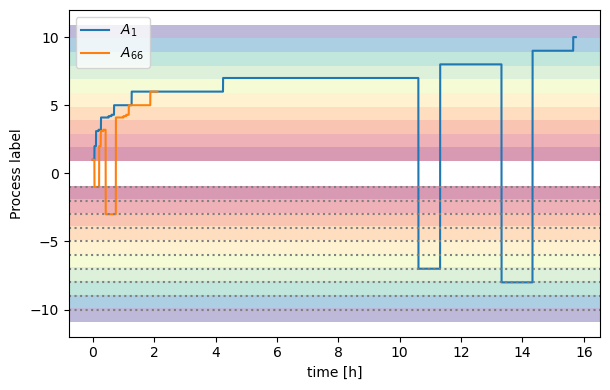
\includegraphics[width=0.8\linewidth]{figures/Multiple cycles data/tailing batch short.png}
    \caption{The first and last batch from cycle A. It is clear that the final batch is cut-off even before the current phase it finished.}
    \label{fig:last batch example}
\end{figure}

After cutting of the final 6 batches, we have a total of 368 batches of which each goes through all the phases. We thus proceed to discuss the negative phase IDs in the following section, where we also discuss the first four phases.




\newpage

\section{Production phases}
This part of the process corresponds to events tagged with ID 1 through 10 but will initially concern itself with ID 1 through 4 as much can be learned from the data set here. In \autoref{fig:B_22 phase 1-4} an example of how the process evolves over time through the different phases is shown. Immediately, we observe something weird, namely the negative event IDs.

\begin{figure}[h]
    \centering
    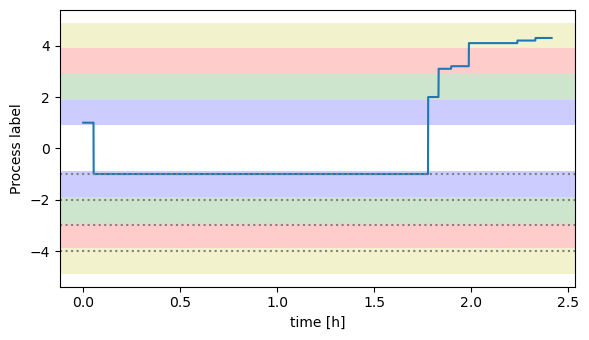
\includegraphics[width=.7\linewidth]{figures/Multiple cycles data/Adding of solids/B_22 long waiting.png}
    \caption{}
    \label{fig:B_22 phase 1-4}
\end{figure}

To see what is going on here, from data we can see that negative values occur throughout all the six cycles. More specifically, for each negative phase observed, we log in which cycles this occurs. The result is shown in \autoref{tab:phase negative observations}. Notice that -4.1, -4.2 and -4.3 only show up in cycle F, which from \cite{benchmark-model-to-generate-batch-process-data} is known to be the only one with wrongly labelled phases. We thus suspect that this is indeed the case for these labels and might just have supposed to be the original 4.1, 4.2 and 4.3. To see if nothing funny goes on with these values, these batches are plotted as in \autoref{fig:B_22 phase 1-4} in \autoref{fig:negative 4 batches}.


\begin{table}[h]
    \centering
    \begin{tabular}{c|c|c|c|c|c|c}
        \diagbox{Event}{Cycle} & A                    & B                    & C                    & D                    & E                    & F                    \\\hline
        -1                     & \cellcolor{black!50} & \cellcolor{black!50} & \cellcolor{black!50} & \cellcolor{black!50} &                      &                      \\\hline
        -2                     &                      &                      &                      & \cellcolor{black!50} & \cellcolor{black!50} & \cellcolor{black!50} \\\hline
        -3                     & \cellcolor{black!50} &                      & \cellcolor{black!50} & \cellcolor{black!50} & \cellcolor{black!50} & \cellcolor{black!50} \\\hline
        -4                     &                      & \cellcolor{black!50} & \cellcolor{black!50} & \cellcolor{black!50} & \cellcolor{black!50} &                      \\\hline
        -4.1                   &                      &                      &                      &                      &                      & \cellcolor{black!50} \\\hline
        -4.2                   &                      &                      &                      &                      &                      & \cellcolor{black!50} \\\hline
        -4.3                   &                      &                      &                      &                      &                      & \cellcolor{black!50} \\\hline
        -5                     & \cellcolor{black!50} & \cellcolor{black!50} & \cellcolor{black!50} & \cellcolor{black!50} & \cellcolor{black!50} & \cellcolor{black!50} \\\hline
        -6                     &                      & \cellcolor{black!50} & \cellcolor{black!50} & \cellcolor{black!50} & \cellcolor{black!50} & \cellcolor{black!50} \\\hline
        -7                     & \cellcolor{black!50} &                      & \cellcolor{black!50} & \cellcolor{black!50} & \cellcolor{black!50} & \cellcolor{black!50} \\\hline
        -8                     & \cellcolor{black!50} &                      & \cellcolor{black!50} & \cellcolor{black!50} & \cellcolor{black!50} & \cellcolor{black!50} \\\hline
        -9                     &                      &                      &                      & \cellcolor{black!50} & \cellcolor{black!50} & \cellcolor{black!50} \\\hline
        -10                    &                      & \cellcolor{black!50} &                      & \cellcolor{black!50} & \cellcolor{black!50} & \cellcolor{black!50}
    \end{tabular}
    \caption{Occurrences of negative phases IDs. It is observed that sub phases 4.1, 4.2, 4.3 only occur in cycle F which is known to be the only cycle with wrongly labelled phases.}
    \label{tab:phase negative observations}
\end{table}



\autoref{fig:negative 4 batches} shows that nothing weird is going on except for the negation of the sub phase's ID. The same can be said for the remaining of the cases where phase ID -4.1, -4.2 and/or -4.3 is used. We thus conclude that these may simply be wrongly labelled thus we convert every such instance to its absolute value and continue with this modified data set from this point on.

\begin{figure}[H]
    \centering
    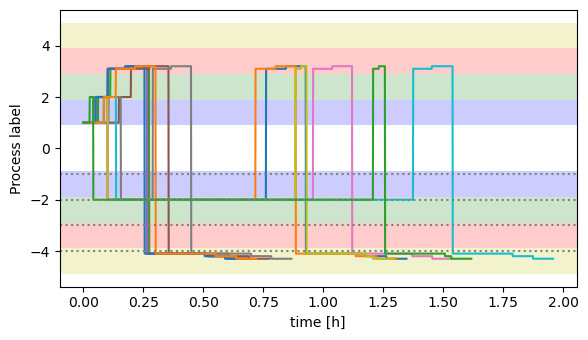
\includegraphics[width=.85\linewidth]{figures/Multiple cycles data/Adding of solids/sample negative sub 4 phases.png}
    \caption{13 of the 48 batches with at least one of the sub phases 4.1, 4.2 4.3 negative.}
    \label{fig:negative 4 batches}
\end{figure}

Having converted the above sub phase IDs we summarize the current situation in regard to negative phase IDs in the following table, \autoref{tab:phase negative observations mod}. Now all the remaining occurrences of negative phase IDS does not seem to exhibit any structure from looking at \autoref{tab:phase negative observations mod}. We thus proceed to understand what is going on with the remaining negative phase IDs.

\begin{table}[h]
    \centering
    \begin{tabular}{c|c|c|c|c|c|c}
        \diagbox{Event}{Cycle} & A                    & B                    & C                    & D                    & E                    & F                    \\\hline
        -1                     & \cellcolor{black!50} & \cellcolor{black!50} & \cellcolor{black!50} & \cellcolor{black!50} &                      &                      \\\hline
        -2                     &                      &                      &                      & \cellcolor{black!50} & \cellcolor{black!50} & \cellcolor{black!50} \\\hline
        -3                     & \cellcolor{black!50} &                      & \cellcolor{black!50} & \cellcolor{black!50} & \cellcolor{black!50} & \cellcolor{black!50} \\\hline
        -4                     &                      & \cellcolor{black!50} & \cellcolor{black!50} & \cellcolor{black!50} & \cellcolor{black!50} &                      \\\hline
        -5                     & \cellcolor{black!50} & \cellcolor{black!50} & \cellcolor{black!50} & \cellcolor{black!50} & \cellcolor{black!50} & \cellcolor{black!50} \\\hline
        -6                     &                      & \cellcolor{black!50} & \cellcolor{black!50} & \cellcolor{black!50} & \cellcolor{black!50} & \cellcolor{black!50} \\\hline
        -7                     & \cellcolor{black!50} &                      & \cellcolor{black!50} & \cellcolor{black!50} & \cellcolor{black!50} & \cellcolor{black!50} \\\hline
        -8                     & \cellcolor{black!50} &                      & \cellcolor{black!50} & \cellcolor{black!50} & \cellcolor{black!50} & \cellcolor{black!50} \\\hline
        -9                     &                      &                      &                      & \cellcolor{black!50} & \cellcolor{black!50} & \cellcolor{black!50} \\\hline
        -10                    &                      & \cellcolor{black!50} &                      & \cellcolor{black!50} & \cellcolor{black!50} & \cellcolor{black!50}
    \end{tabular}
    \caption{Occurrences of negative phases IDs. It is observed that sub phases 4.1, 4.2, 4.3 only occur in cycle F which is known to be the only cycle with wrongly labelled phases.}
    \label{tab:phase negative observations mod}
\end{table}

When plotting different batches, it is clear that the negative phase IDs only occur at the end of a phase e.g. -1 only happens after 1 and so on. This together with the fact that -3 and -4 also only happen after 3.1, 3.2 and 4.1, 4.2, 4.3 respectively (and we never see a phase labelled 3 or 4) indicate that the negative phase IDs could very well correspond to delays at the end of a phase, which both makes sense from a production point of view but also from \cite{benchmark-model-to-generate-batch-process-data} where they note that all simulated cycles have been implemented with delays.

At this point, it would seem that the labels of the processes are understood for phases 1 through 10 corresponding to the actual production in each batch. Thus, we proceed by searching relationships and otherwise quantifying the durations of each phase, both delays and duration for each of the phases. As a beginning, histograms for each of the phases and delays are plotted in \autoref{fig:histogram production durations}. Notice that phases 4.1, 4.3 and 8 are not shown, this is because they always last 15 min, 5 min and 2 hours respectively with the only derivation being in machine precision either when loaded or during calculations. Furthermore, notice that for the negative IDs i.e. the delays, the orange bar. This bar represents the cases where no delay was observed which is thus modelled as an atom at 1.

\begin{figure}[H]
    \centering
    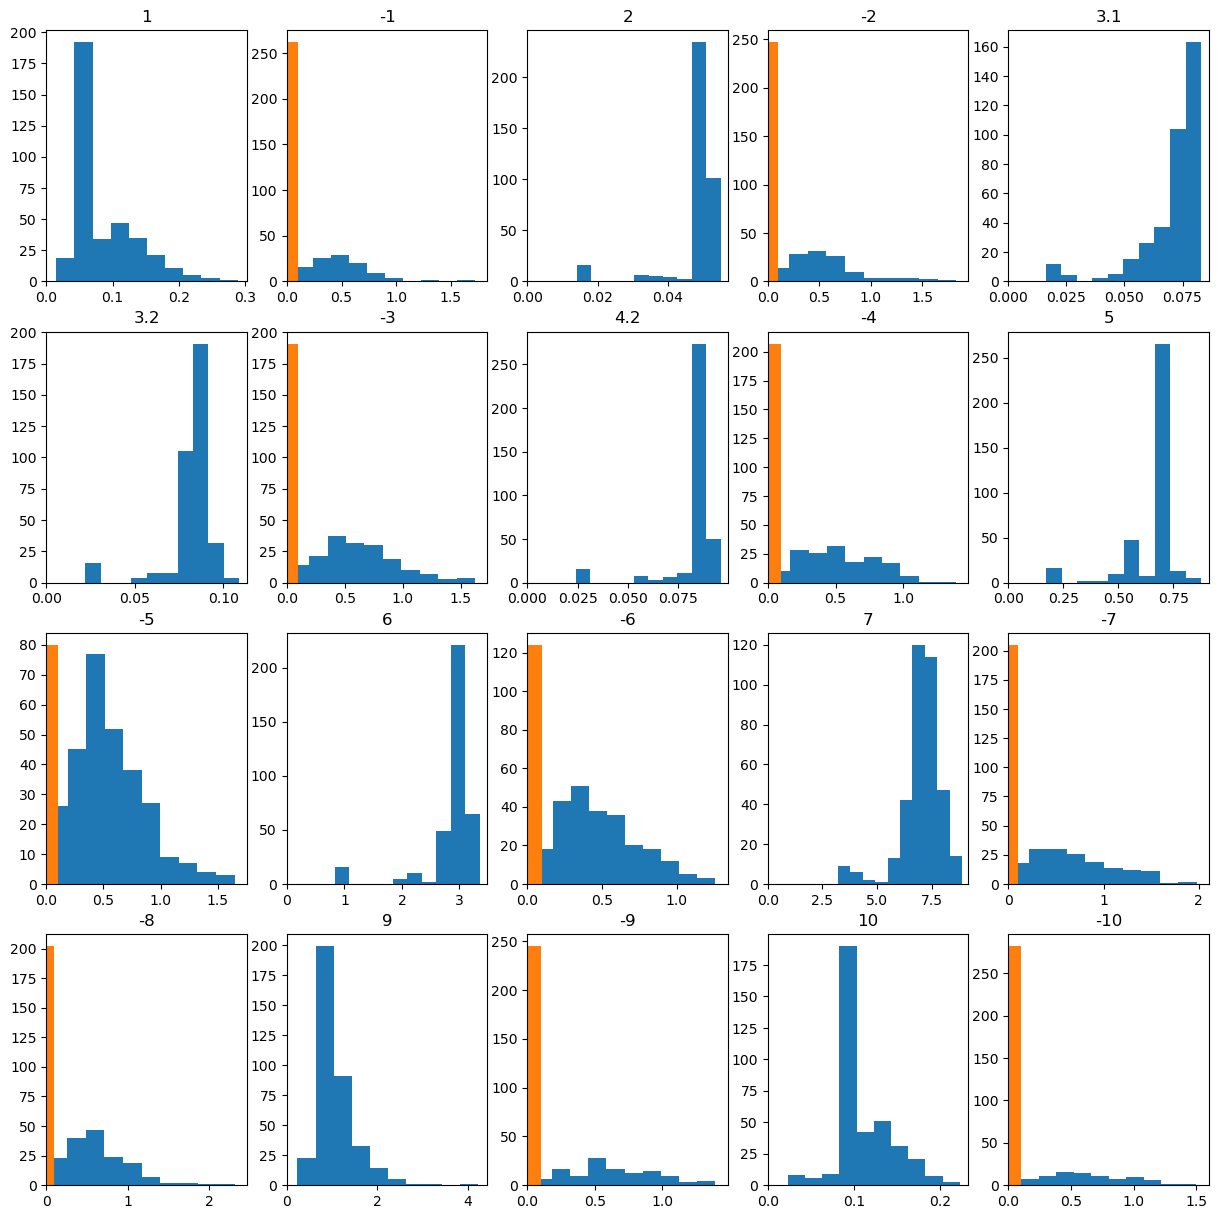
\includegraphics[width=\linewidth]{figures/Multiple cycles data/Adding of solids/hisstograms w atoms.png}
    \caption{Histograms of all phases and delays which are non-constant.}
    \label{fig:histogram production durations}
\end{figure}

Apart from the above comments, not much catches the eye when looking at \autoref{fig:histogram production durations}, and we thus proceed by checking if any correlation is immediately present.




\subsection{Correlations}

Lige en korrelationsmatrix
\begin{figure}[H]
    \centering
    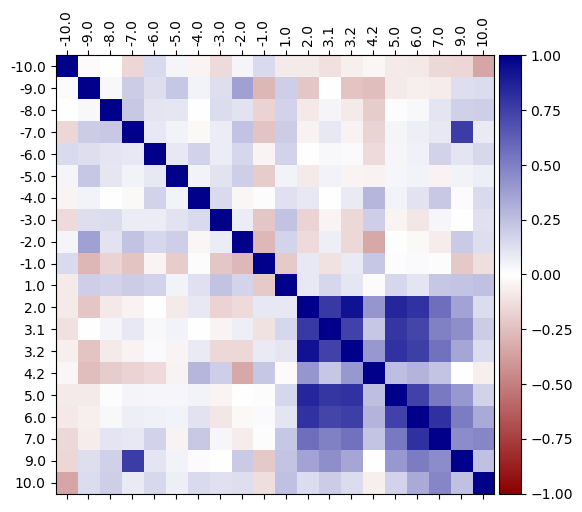
\includegraphics[width=.9\linewidth]{figures/Multiple cycles data/Correlation matrix production and delays.png}
    \caption{Correlation matrix for all phases with non-constant duration.}
\end{figure}

9 og 10 er ikke specielt korreleret med noget (afkøling og materiale overførsel). Ellers er 2 fremt il og med reaktionen alle korrelerede med hinanden. Eftersom rent fysisk det udvikles i tid, må handlingen i 2 påvirke de næste osv.

\begin{figure}
    \centering
    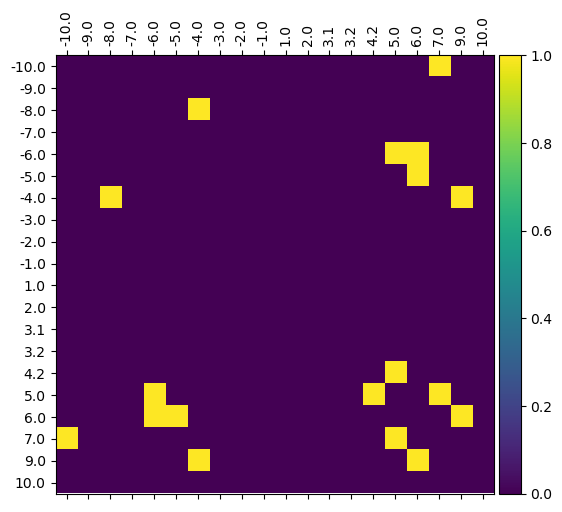
\includegraphics[width=.9\linewidth]{figures/Multiple cycles data/Permutation test rho 10 mil.png}
    \caption{Permuteringstest med $\alpha = 0.05$. Also run with less simulations but same result at 1 mil and 10k sims. The Benjamin-Hochberg procedure on the upper (or lower) triangle reveals that none of the correlations are significant.}
\end{figure}

Umiddelbart lidt spøjst hvis delay på 7 (reaktion) skulle have noget med tiden for afkøling at gøre, især at den skulle være positiv (ville man ikke tro delay efter produktion ville afkøle mere og dermed reducere behov for afkøling, medmindre varmt steam bliver tilføjet også under delay på 7)




Herunder er samme korrelationsmatrix, dog hvor delay og phasens varighed lagt sammen (også med sub phases såsom 3.1, 3.2 og -3 tilsammen bliver 3)

\begin{figure}[H]
    \centering
    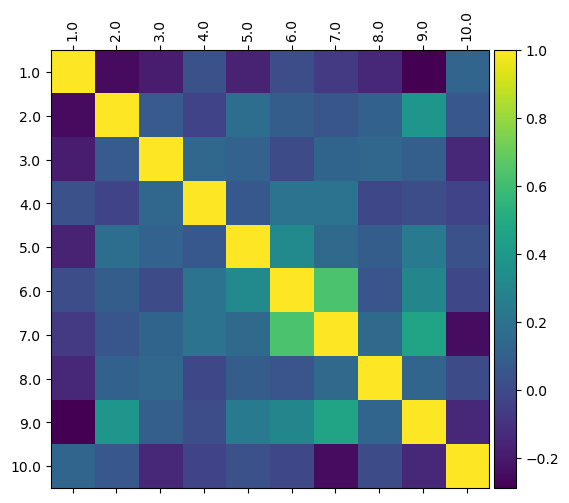
\includegraphics[width=.7\linewidth]{figures/Multiple cycles data/Correlation matrix collapsed phases.png}
    \caption{Correlation matrix for all phases collapsed}
\end{figure}


Ligeledes scatter plots for superdiagonalen i ovenstående matrix. Altså phase 1 overfor phase 2, phase 2 overfor phase 3 osv. Er farvelagt efter hvilken cycle de kommer fra. \autoref{tab:phase negative observations mod} forklarer hvorfor nogle af de horisontale fremkommer sammen med \autoref{fig:histogram production durations} (selve produktionstiden er ret kort sammenlignet med delay.)
\begin{figure}[H]
    \centering
    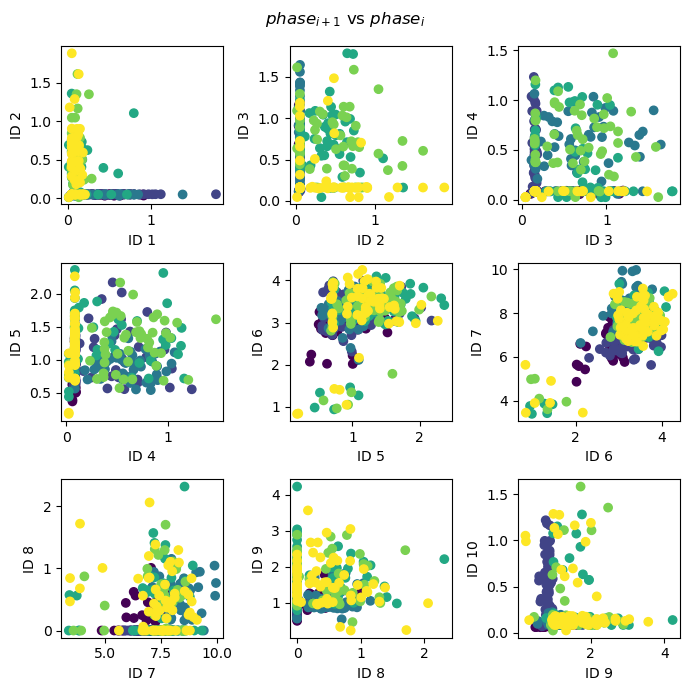
\includegraphics[width=\linewidth]{figures/Multiple cycles data/phase scatter vs next phase.png}
    \caption{Phases vs their next phase when collecting everything regarding a single phase into a total time duration}
\end{figure}



% Check at eventID altid er kronologisk stigende, absolut værdi (med undtagelse for 3 og 4, der gør lidt tilbage grundet waiting time)

% Peaks i e.g. 1, kommer det fra en specifik cycle?

% sammenhæng med fyldningsniveau?

% correlaiton diagrammer

% Betyder delay på 7 (ID -7) at der bliver produceret mere? Eller er det bare den er færdig og man så venter til næste operation?

% Skal man måske prøve at modellere sig ud af korrelationen? Måske ved at kigge på fyldningsniveauet, da det nok beskriver en del


\newpage
\section{Cleaning operations}
Sometimes, the vessel is cleansed. This is however not every time after a batch so might be interesting to investigate further. Initially, per cycle, the cleanings are summarized in the following table with basic statistics. As can be seen, there is quite some differences.

The most notifiable differences per batch are the number of cleanses especially when comparing to \autoref{tab:cycle basi stats}. For the first two cycles, the cleanses seem to be in between every batch, which is indeed also the while the later four are only sometimes. Furthermore, although the cleanses are between every batch for cycles A and B, the variances are extremely different. For the last four cycles, they seem to be grouped further, E and F are very alike while cleanses in C and D are generally longer although D has a substantially smaller variance than C.

\begin{table}[h]
    \centering
    \begin{tabular}{c|c|c|c|c|c|c|c}
        Cycle & \#ops & min   & max   & $\mu$ & $\sigma^2$ & $\sigma$ & $\sigma / \mu$ \\ \hline
        A     & 65    & 1.113 & 3.067 & 1.917 & 0.269      & 0.518    & 0.270          \\
        B     & 63    & 1.324 & 1.751 & 1.566 & 0.00883    & 0.0939   & 0.0600         \\
        C     & 9     & 1.544 & 3.306 & 2.153 & 0.277      & 0.526    & 0.245          \\
        D     & 10    & 1.474 & 2.009 & 1.581 & 0.0212     & 0.146    & 0.0922         \\
        E     & 10    & 0.827 & 1.584 & 1.465 & 0.0462     & 0.215    & 0.147          \\
        F     & 10    & 0.748 & 1.610 & 1.466 & 0.0595     & 0.244    & 0.166
    \end{tabular}
    \caption{Per cycle cleansing statistics}
    \label{tab:cycle cleansing stats stats}
\end{table}

To verify these observations and potentially discovering more important facts of their probability distributions, histograms are plotted in the following \autoref{fig:cycle cleaning histograms}. We indeed again observe the likeliness between the cycles A and B, C and D, E and F respectively. Also, for the first two cycles and more so cycle B, the cleaning times are somewhat normally distributed although cycle A has a very heavy right tail in that case. The later four cycles only have 10 observations but the mode (i.e. peak) seem to be about the same.

\begin{figure}[h]
    \centering
    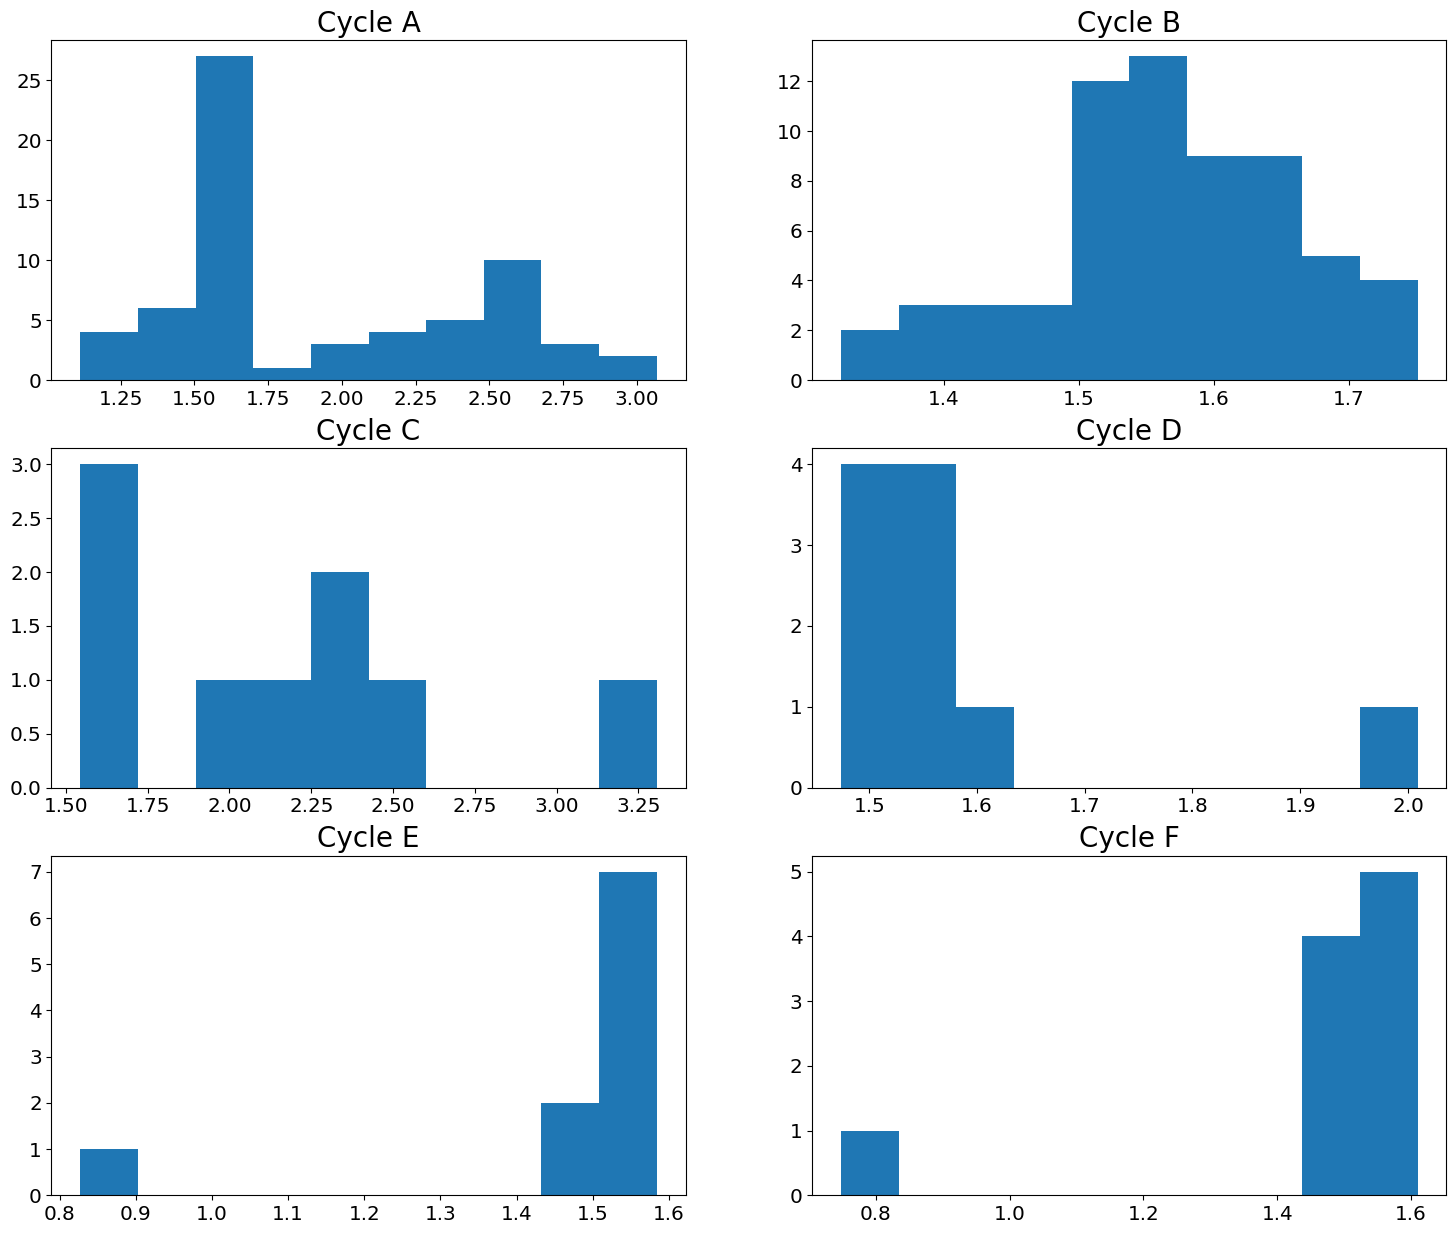
\includegraphics[width=0.8\linewidth]{figures/Multiple cycles data/Cleaning batches histograms.png}
    \caption{Each of the 6 cycles, cleaning operations histograms.}
    \label{fig:cycle cleaning histograms}
\end{figure}

From the above observation of like modes one may want to observe the histogram of the combined set of cleaning times. In particular, under the hypothesis that the durations are actually from the same probability distributions and realized independently within each cycle a histogram of all the observations are of interest and is shown in \autoref{fig:cycle cleaning histograms combined} below.


\begin{figure}[H]
    \centering
    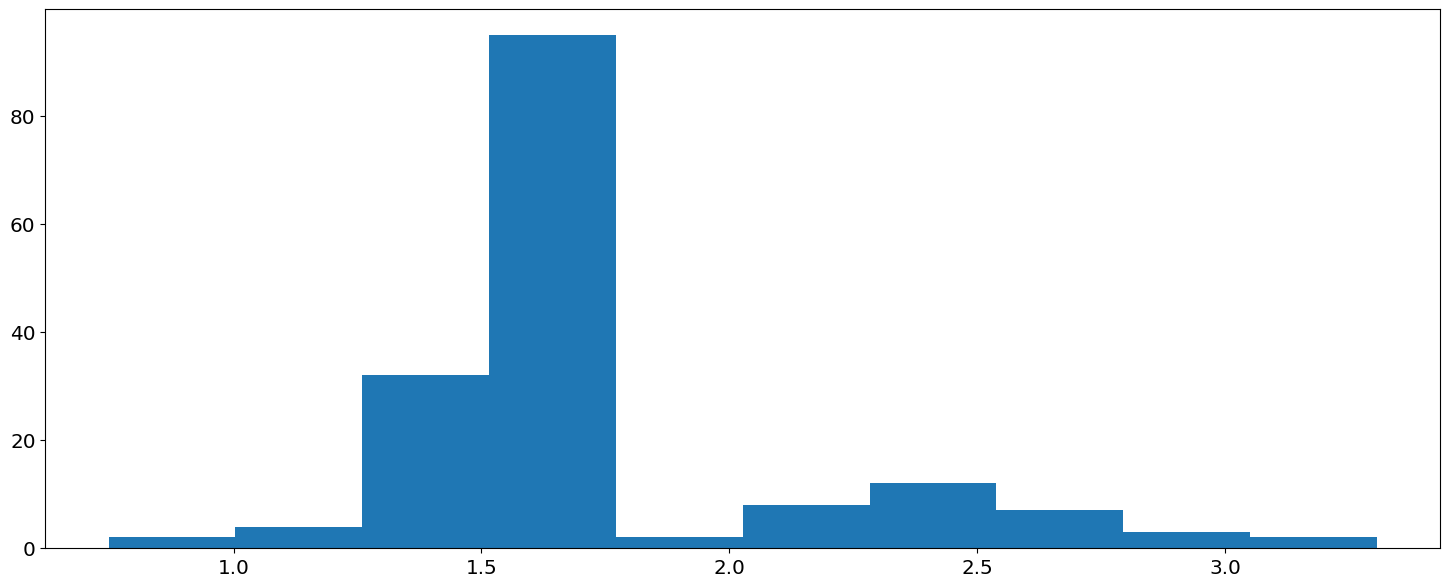
\includegraphics[width=0.8\linewidth]{figures/Multiple cycles data/Cleaning batches histograms combined.png}
    \caption{Combined cleaning operations histograms.}
    \label{fig:cycle cleaning histograms combined}
\end{figure}


Finally, to get a better overview of the irregularities is the number of cleaning periods (mostly concerning cycles C through F), each cleaning operation is shown in the following \autoref{fig:cycle cleaning time series}. The vertical shaded rectangles signify the period in which a cleaning operation is taking place. Furthermore, the event IDs are shown but to get a clearer view on what is going on, a single rectangle (zoomed in) is shown in \autoref{fig:cycle cleaning time series single}.

\begin{figure}[H]
    \centering
    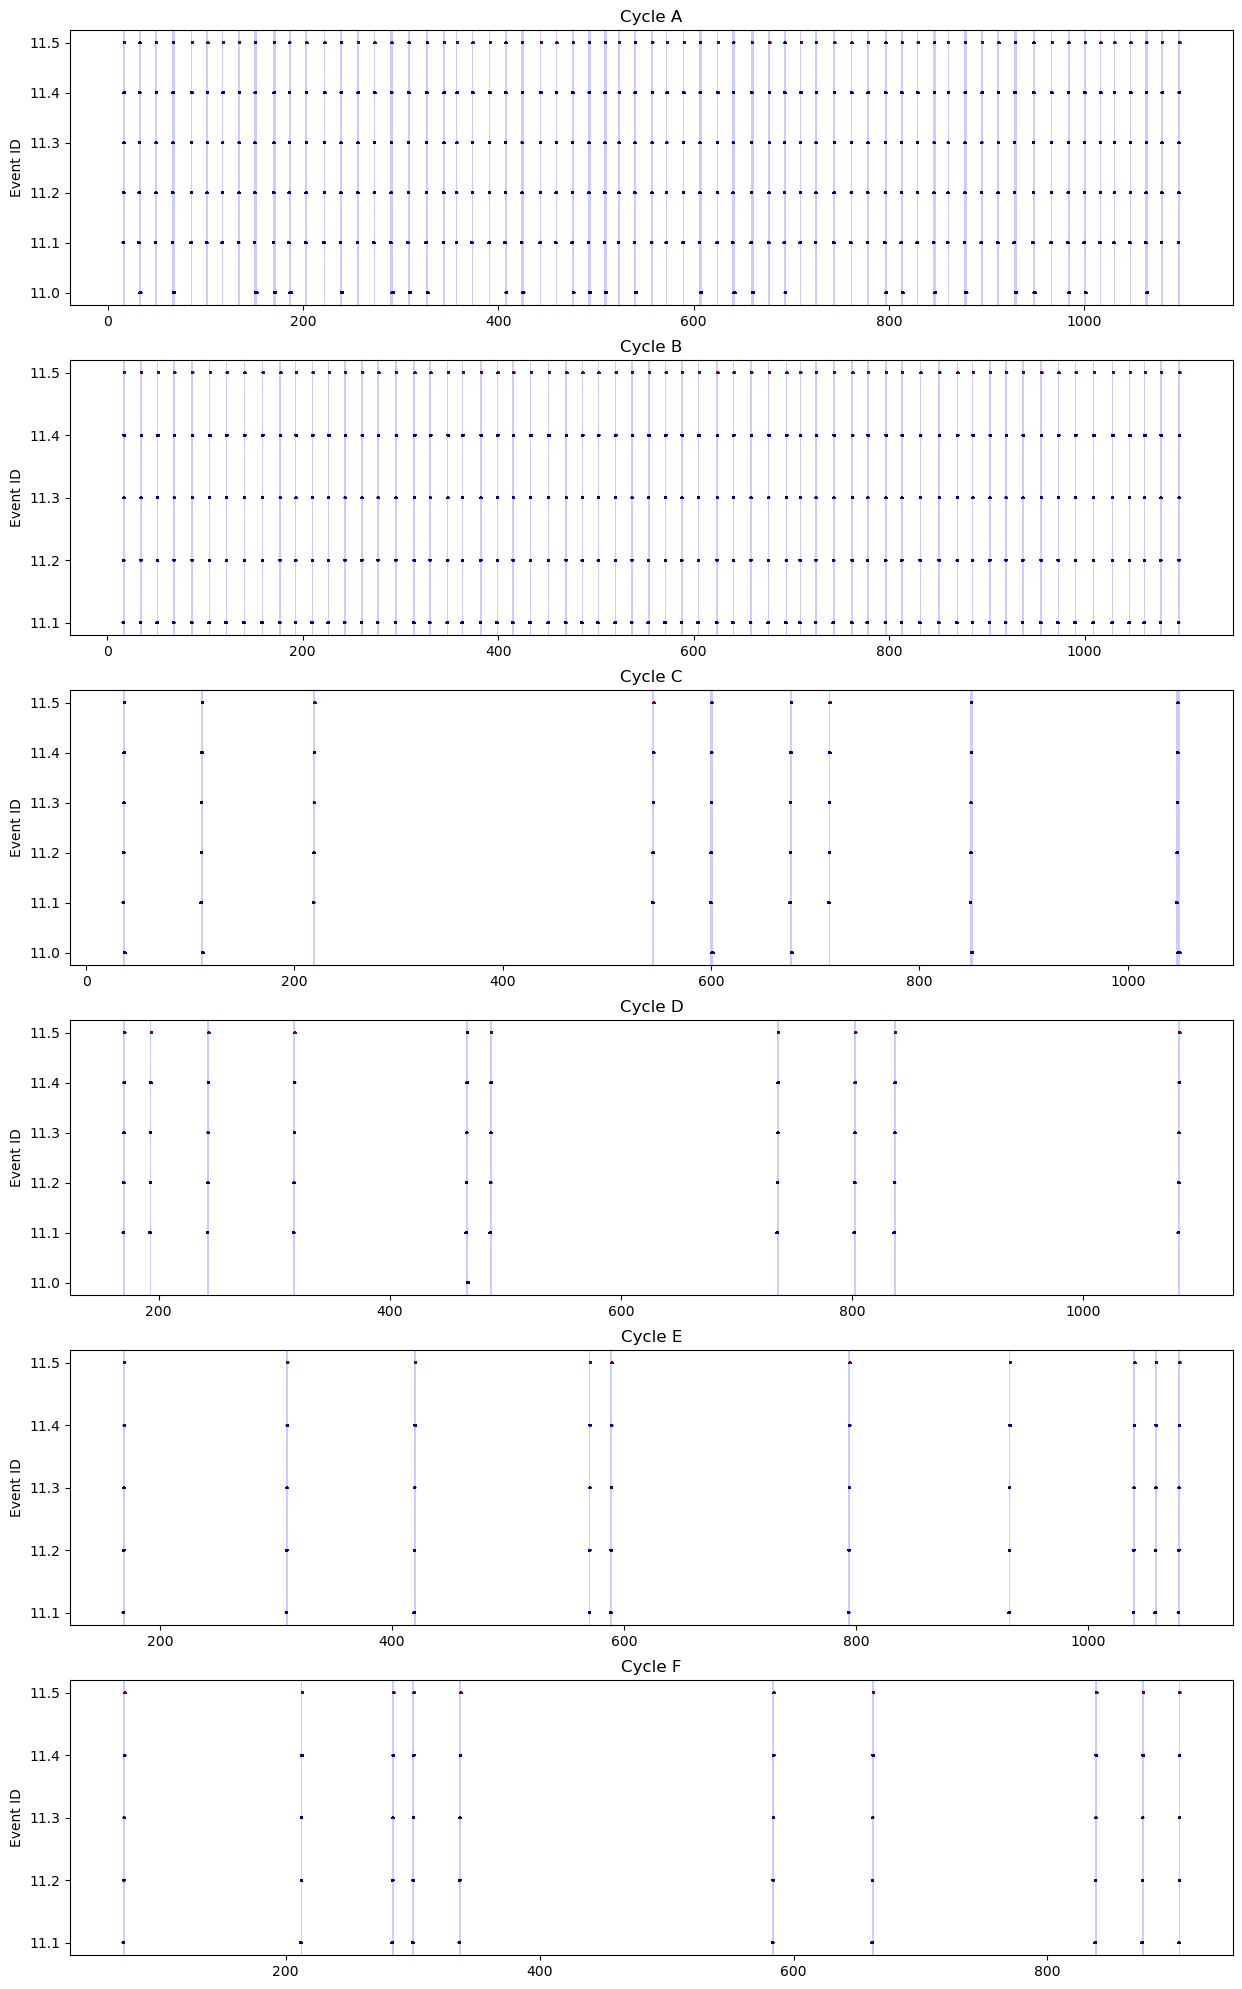
\includegraphics[width=0.9\linewidth]{figures/Multiple cycles data/Cleaning batches.png}
    \caption{Each of the 6 cycles, cleaning (corresponding to \texttt{BatchID = 0}). Each \textit(Cleaning Procedure), CIP, is highlighted with an opaque interval (the blue rectangles). The dots marked with red (only ID 11.5, but not all of these are red), is if the Cleaning ID is 0.}
    \label{fig:cycle cleaning time series}
\end{figure}


\begin{figure}[h]
    \centering
    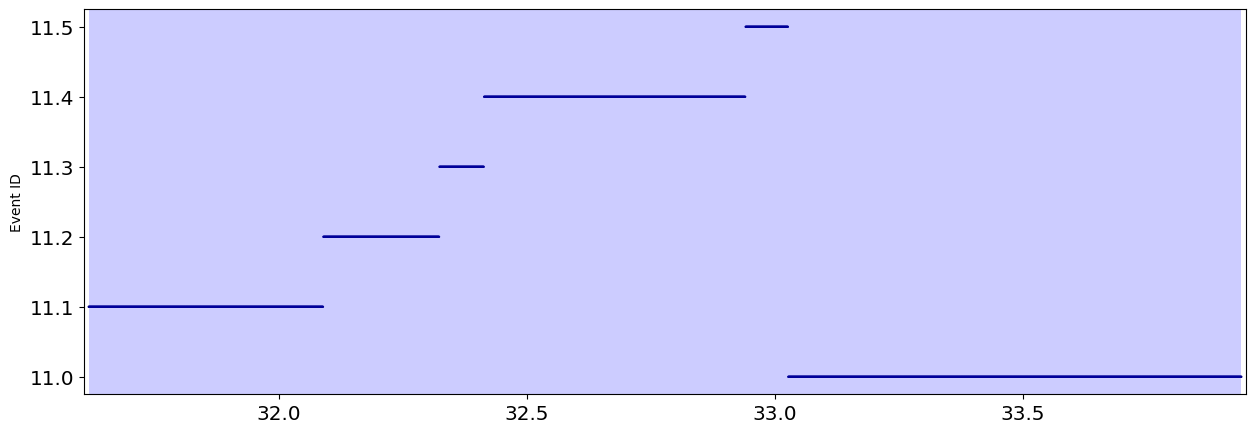
\includegraphics[width=0.9\linewidth]{figures/Multiple cycles data/Cleaning batches timeseries single.png}
    \caption{A single blue rectangle zoomed in}
    \label{fig:cycle cleaning time series single}
\end{figure}

It is observed that the observations marked with red in figure \ref{fig:cycle cleaning time series} occur exactly when that specific cleaning operation does not go to the state 11.0 after the flush of the tank (event ID 11.5) and vice versa. It is hard to conclude what this may mean, but the cleaning being in state 11.0 may indicate that the system is idle before continuing the next batch like what is observed from the other steps of the process flow. Also, it is noted that while the red dots occur nothing else is happening according to the dataset.


From a modelling point of view, the cycles C through F can be thought of as the cleansing operation having a probability of not happening or equivalently as having a duration of 0. It is thus of interest to observe what the probability of cleaning after an operation is. From \autoref{tab:cycle basi stats} and \autoref{tab:cycle cleansing stats stats}, we that indeed for cycles A and B, the probability is 100 \% when disregarding the possibility of cleaning after the final batch. Hence, we see that for the remaining cycles, the probabilities of cleaning the tank after an operation are as in \autoref {tab:cycle cleaning prob}

\begin{table}[h]
    \centering
    \begin{tabular}{c|r}
        Cycle & \% cleaning \\ \hline
        A     & 100.00      \\
        B     & 100.00      \\
        C     & 15.00       \\
        D     & 16.95       \\
        E     & 16.95       \\
        F     & 16.13
    \end{tabular}
    \caption{Per cycle probability of cleaning}
    \label{tab:cycle cleaning prob}
\end{table}


Furthermore, let $C_i$ denote whether the $i$th batch is followed by a cleaning of the tank or not. It is then of interest if the next batch is followed by a cleaning given whether the current batch is followed by a cleaning. In particular, we count for each of the cycles the transitions which are shown in the following tables. Notice that the number of observations is two less than the total number of batches within each specific cycle. This is due to the last batch is never followed by a cleaning (nor is the first batch superseded by a cleaning procedure) which results in one less observation and also due to the fact that we are logging transitions and hence lose another observation. To test for randomness, a Chi-squared test is carried out on each of the cycles to check for independence. It is observed all the cycles exhibit independence between the groups i.e. there is no statistical evidence for information is gained about if the next batch is followed by a cleaning operation given whether the current batch is followed by a cleaning operation.

\begin{table}[h]
    \begin{subtable}{.5\linewidth}
        \centering
        \begin{tabular}{c|c c}
            \diagbox{$C_i$}{$C_{i+1}$} & No & Yes \\ \hline
            No                         & 41 & 9   \\
            Yes                        & 9  & 0
        \end{tabular}
        \caption{C, $p=0.3293$}
        \label{tab:cycle C Contingency table}
    \end{subtable}%
    \begin{subtable}{.5\linewidth}
        \centering
        \begin{tabular}{c|c c}
            \diagbox{$C_i$}{$C_{i+1}$} & No & Yes \\ \hline
            No                         & 41 & 8   \\
            Yes                        & 7  & 2
        \end{tabular}
        \caption{D, $p=0.6456$}
        \label{tab:cycle D Contingency table}
    \end{subtable}
    \begin{subtable}{.5\linewidth}
        \centering
        \begin{tabular}{c|c c}
            \diagbox{$C_i$}{$C_{i+1}$} & No & Yes \\ \hline
            No                         & 41 & 7   \\
            Yes                        & 7  & 3
        \end{tabular}
        \caption{E, $p=0.3532$}
        \label{tab:cycle E Contingency table}
    \end{subtable}%
    \begin{subtable}{.5\linewidth}
        \centering
        \begin{tabular}{c|c c}
            \diagbox{$C_i$}{$C_{i+1}$} & No & Yes \\ \hline
            No                         & 41 & 9   \\
            Yes                        & 9  & 1
        \end{tabular}
        \caption{F, $p=1.0000$}
        \label{tab:cycle F Contingency table}
    \end{subtable}

    \caption{Contingency table for Cycle C-F}
    % \label{tab:}
\end{table}

Thus collecting the observations from all the last four cycles, we may want to model the atom of the cleaning procedure independently of the previous batch and with a probability of $0.8375$ corresponding to the cleaning procedure only being carried out $16,25$\% of cases.

Finally, we show the autocorrelation function for each the four cycles C-F in \autoref{fig:cycle cleaning ACF} and note that all the ACF stay within the 95\% confidence interval.

\begin{figure}[h]
    \centering
    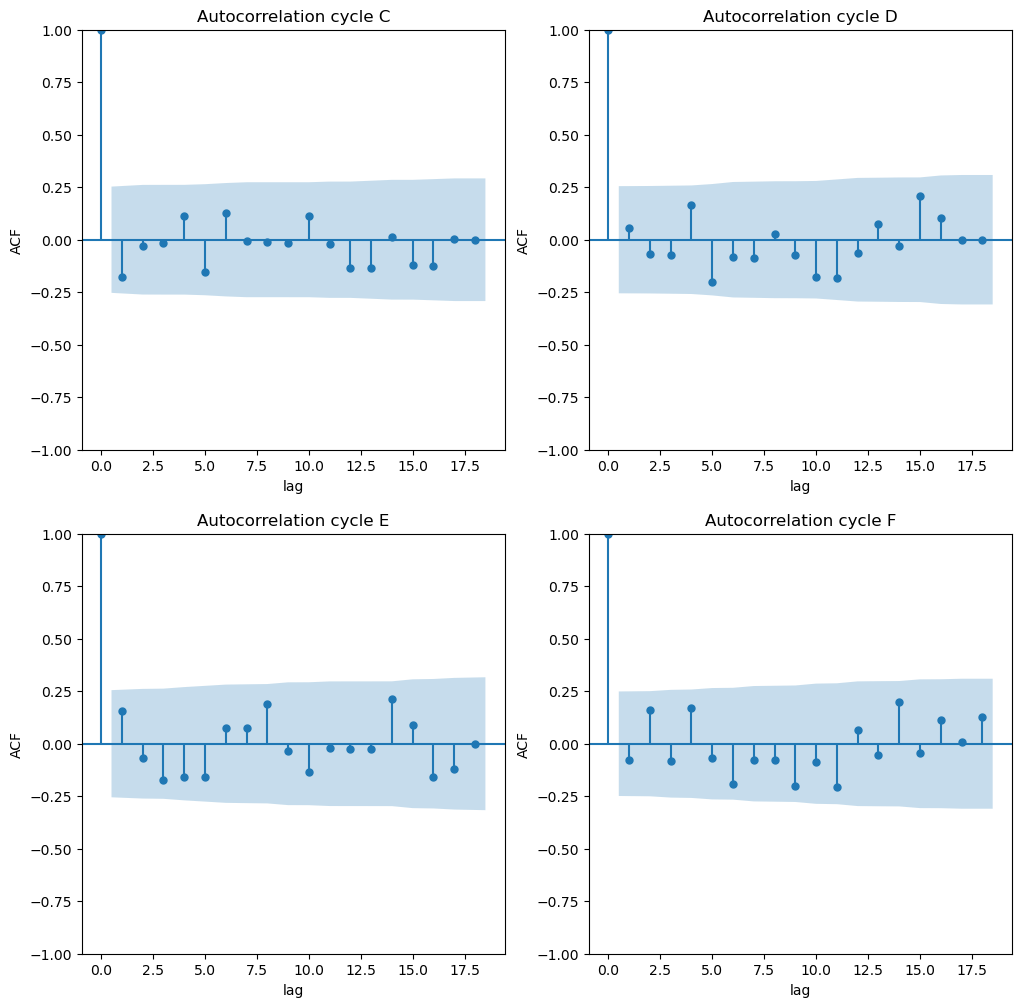
\includegraphics[width=0.8\linewidth]{figures/Multiple cycles data/Cleaning Autocorrelation.png}
    \caption{Autocorrelation function for each of the final 4 cycles. As can also be seen from this there seem to be no information to be gained of $C_i$ from $C_{i-1}$.}
    \label{fig:cycle cleaning ACF}
\end{figure}

\end{document}


% There is a relationship between the red dots and when the cleaning does not \textit{return} to state 11.0 -> probably no


% Correlationssky mellem delay og % filled




% 1 og -1 sammen osv -> ny korrelationsmatrix -> DONE

% Binært billede af korrelationsmatrix om hvad der er med ud fra threshhold T (varirer lidt om hvad der kan give mening -> absolutværdi af korrelation obv.))

% plot tider for operationer over for hinanden: O1 vs O2, O2 vs O3 -> DONE



% Bo skal sende Claras PhD. vedrørende togmodeller

% MODEL: baseret på threshhold for en phase, kan gå to veje, MPH* mmodel i den ene (måske) , MPH* i den anden + hale (eksponentiel)


% CME ILT TELEK

% undersøg delay propagation - artikler


% se på kurver om der sker noget specielt under negative event med fyldningsniveauer